% !TEX encoding = UTF-8
% !TEX TS-program = pdflatex
% !TEX root = ../tesi.tex
% !TEX spellcheck = it-IT

%**************************************************************
\chapter{Valutazione Retrospettiva}
\label{cap:valutazione-retrospettiva}
%**************************************************************
\intro{Questo capitolo riporta un bilancio finale su quanto svolto durante lo stage.}




%**************************************************************************************************
\section{Bilancio sui risultati}
In questa sezione riassumo gli obiettivi aziendali e gli obiettivi personali raggiunti durante lo stage.
\subsection{Obiettivi conseguiti}
Gli obiettivi fissati all'inizio dello stage, hanno subito delle modifiche. L'azienda ha voluto privilegiare il \emph{\gls{portingg}} di DRE. Il \emph{\gls{portingg}} dell'applicativo è parzialmente completato. L'unica funzionalità non ancora implementata è una procedura di \emph{map-reduce}. Questa funzionalità non l'ho completata, perché le mie competenze per comprendere quel codice erano insufficienti. Le parti su cui intervenire erano scritte in javascript, sistemarle avrebbe introdotto un ulteriore ritardo per lo sviluppo di Tres. L'obiettivo di migliorare la fase di apprendimento di questo modulo non l'ho raggiunto. Durante lo sviluppo di Tres ho individuato 23 requisiti, di cui, come raffigurato in \ref{fig:graficorequisiti}, 20 obbligatori e 3 desiderabili.  
\begin{figure}[h]
\centering
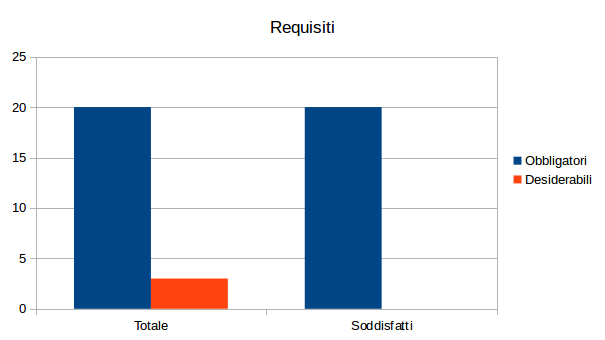
\includegraphics[scale=0.64]{immagini/graficorequisiti}
\caption{Riassunto requisiti}
\label{fig:graficorequisiti}
\end{figure}
\\I requisiti desiderabili non soddisfatti riguardavano l'implementazione di algoritmi di \emph{clustering}, pertanto questo scopo non è stato raggiunto.
Tuttavia ho raggiunto l'obiettivo di implementare algoritmi per l'individuazione dei gusti dell'utente, grazie all'implementazione di \emph{ID3}. In questo stage ho conseguito il \emph{target} minimo riguardante l'utilizzo di OrientDb. Durante le due attività di \emph{\gls{portingg}} e sviluppo, ho avuto modo di utilizzare questa tecnologia. 
\subsection{Obiettivi personali}
All'inizio dello stage, il mio scopo era di imparare nuove tecnologie da aggiungere alle mie conoscenze. Ritenevo il mio bagaglio professionale insufficiente, per affrontare il mondo del lavoro. Lo stage mi ha permesso di padroneggiare molte tecnologie, quali: OrientDb, Scala e un \emph{web \gls{framework}} di concezione moderna. Scala mi ha dato la possibilità di apprendere le nozioni per un corretto stile di programmazione funzionale. Mi ero prefissato di approfondire argomenti quali, intelligenza artificiale e i sistemi di raccomandazione. Ritengo questo parzialmente soddisfatto. Non ho trovato il supporto necessario per approfondire queste competenze, soprattutto per i sistemi di raccomandazione.
%**************************************************************************************************




%**************************************************************************************************
\section{Bilancio formativo}
In questa sezione riporto le competenze acquisite durante lo stage.\\
Lo stage in Nextep Srl è stata la  mia prima esperienza nel settore informatico. Mi ha permesso di apprendere nuove competenze e consolidare competenze già apprese durante il corso di studi.
%Prima avevo idee molto confuse a riguardo la mia carriera professionale, ma ora dopo lo stage posso affermare di avere aspettative più ambiziose e idee più chiare su quale cammino professionale intraprendere.
Ho trovato molto positivo lavorare collaborativamente al progetto, perché questo mi ha portato a migliorare le mie capacità di \emph{team working}. Questa abilità è molto importante nel mondo del lavoro, soprattutto nei contesti lavorativi dove si utilizza una metodologia \emph{agile}. Ho migliorato le mie capacità di \emph{project management} per concludere il progetto nei tempi fissati e raggiungere gli obbiettivi minimi che mi sono prefissato. In conclusione, ho terminato lo stage con un bagaglio professionale più ricco e di essere in grado di farmi carico di responsabilità più importanti.
\newpage
\subsubsection{Scala}
Durante lo stage ho avuto modo di apprezzare i vantaggi derivanti dall'uso di questo linguaggio. Ho utilizzato questa tecnologia nelle attività di \emph{\gls{portingg}} del modulo DRE e nell'attività di sviluppo di Tres. Per studiare Scala ho seguito un corso \emph{online}\footcite{https://www.coursera.org/course/progfun} tenuto direttamente dal professore Martin Odersky\footcite{http://lampwww.epfl.ch/~odersky/}, ovvero il \emph{designer} del linguaggio stesso. Un corso validissimo per capire i meccanismi e le peculiarità di questo linguaggio. All'inizio è stato un po' ostico mettere in pratica quanto appreso, ma quando ho cominciato a padroneggiare Scala ho potuto constatare un aumento della mia produttività. Ho trovato un po' macchinoso gestire la compatibilità con librerie Java di terze parti. Mi ritengo soddisfatto di aver imparato questa tecnologia e di poter reinvestire nel mondo del lavoro questa conoscenza. 
Scala mi ha introdotto al paradigma di programmazione funzionale. Questo paradigma mi ha fornito una modalità diversa di affrontare e risolvere problemi, rispetto alla classica programmazione orientata agli oggetti. Nella programmazione funzionale vengono evitati i dati di stato e modificabili, mentre viene data invece una maggiore enfasi all'applicazione di funzioni. Mantenere gli stati immutabili facilita la suddivisone del codice per l'esecuzione parallela, garantendone la correttezza. Questa caratteristica è importantissima al giorno d'oggi, dove il focus si sta via via spostando sempre di più verso contesti multi-threading. %Per concludere questo paradigma induce ad uno stile di programmazione più espressivo e conciso 
\subsubsection{OrientDb}
Questa tecnologia è la soluzione di persistenza adottata durante il progetto. La curva di apprendimento è stata molto rapida, grazie al corso online\footcite{https://www.udemy.com/orientdb-getting-started/}, tenuto durante l'attività di formazione. Mi ha permesso di imparare le differenze tra i modelli più tradizionali, come i relazionali e i modelli a grafo. I modelli a grafo si prestano molto bene per soluzioni nel dominio web, soprattutto in questo momento storico, dove il web si sta evolvendo in web semantico. E' stato un po' difficoltoso all'inizio passare dal concetto di \emph{Join} delle tabelle al concetto di \emph{Traverse} dei grafi. Tuttavia la modellazione del dominio con un grafo, è stata molto più semplice ed intuitiva rispetto ad un modello relazionale. 
\subsubsection{Play Framework}
L'apprendimento di questo \emph{framework} non è particolarmente difficile. La documentazione presente nel sito è molto esaustiva, fornisce un supporto completo per la configurazione di una web application. Trovo molto vantaggioso la compatibilità con i linguaggi Java e Scala, in modo da poter sviluppare una applicazione con entrambi i linguaggi. La prima configurazione iniziale è stata molto semplice, questo mi ha permesso di focalizzarmi subito nello sviluppo del modulo. Purtroppo ho trovato complicato testare parti del mio modulo, perché  era necessario, per il test, avere l'istanza del server avviata.
%**************************************************************************************************




%**************************************************************************************************
\newpage
\section{Distanza tra formazione universitaria e lavoro}
In questa sezione espongo la valutazione personale, della distanza tra la formazione ricevuta durante il corso di studi e lo stage formativo. 
%Questa esperienza mi ha permesso di valutare la distanza tra la formazione universitaria e le competenze realmente richiesta durante lo stage.
L'insegnamento che mi ha maggiormente preparato ad affrontare lo stage, è sicuramente \emph{Ingegneria del Software}.
Le competenze mancanti ad inizio stage non sono state molte.
Il \emph{gap} formativo è stato adeguato per essere colmato durante le attività svolte. Soprattutto durante l'attività di studio della prima settimana, che mi ha permesso di apprendere le conoscenze necessarie per affrontare le attività successive.\\
L'attività di modellazione del \emph{database} è stata una delle difficoltà maggiori incontrata durante il percorso. La modellazione di una base di dati a grafo, richiede un approccio differente al problema rispetto alle soluzioni relazionali.\\
Una difficoltà minore riguarda la programmazione funzionale. Questo paradigma all'inizio mi è risultato difficoltoso da assimilare, perché abituato ai linguaggi orientati agli oggetti.\\
Uno strumento che ho spesso utilizzato e che non è stato introdotto durante il corso di studi, è il debugger. Questo strumento risulta molto utile, per individuare errori e comportamenti non attesi del codice.\\
Durante lo stage, mi sono mancate le nozioni base per implementare fedelmente una architettura \gls{rest}. Questa tecnologia l'ho già affrontata, durante il progetto finale di ingegneria del software. Ma non è stato sufficiente per assimilarne la filosofia di base.\\
Per concludere le mie lacune più evidenti, sono fondamenti di intelligenza artificiale e i sistemi di raccomandazione. Avere queste nozioni all'inizio dello stage, mi avrebbe sicuramente aiutato durante analisi dei requisiti per il modulo Tres. L'attività di analisi, infatti, è stata in assoluto la difficoltà maggiore. Conoscere il dominio, mi avrebbe permesso di intercettare con più efficacia le esigenze del proponente.
%GIA PREVISTO testing del codice più efficace -> questa abilità è qualificante
%GIA PREVISTO capacità di progettare una architettura flessibile, --> poca enfasi nei design pattern
%GIA PREVISTO NEL CORSO team working -> prevedere più progetti di gruppo
%GIA PREVISTO abilità nel \gls{portingg} dell'applicativo -> introdurre delle best practice


%Per concludere, programmazione asincrona
% fare discorso su debugger????
%L'insegnamento che mi ha maggiormente preparato per questa esperienza, è sicuramente \emph{Ingegneria Del Software}. Grazie a questo corso ho appreso molte nozioni tecniche e un approccio valido per la gestione e la produzione software, un bagaglio molto importante per il mondo del lavoro.
%La prima difficoltà che ho incontrato riguarda l'attività di modellazione del \emph{database}. Mi sarebbe stato utile avere delle nozioni per affrontare una modellazione su di un database a grafo. Durante il corso di \emph{Basi di Dati}, invece, vengono insegnate solamente soluzioni come i \emph{database} relazionali. Sarebbe sufficiente introdurre dei fondamenti sulle varie tipologie di database, in modo che lo studente possa valutare pro e contro di ogni tipologia e utilizzare la soluzione migliore a seconda del contesto.
%Sarebbe utile fornire dei concetti di programmazione funzionale, questo stile di programmazione risulta molto adatto per soluzioni \emph{multi-threading}. Si potrebbe introdurre questi concetti durante il corso di \emph{programmazione concorrente e distribuita}, sempre col medium di Java, in modo sfruttare facilmente il parallelismo offerto dalle odierne architetture.
%A livello tecnico, ritengo che durante il corso di laurea sia dato poco spazio per apprendere e consolidare tecniche di programmazione valide, ed evitare quindi errori comuni in sede lavorativa. Dovrebbero essere introdotti i design pattern e il loro corretto utilizzo durante il corso di \emph{programmazione ad oggetti}.
%Sarebbe importante, nel corso di \emph{Programmazione}, spiegare come utilizzare strumenti per fare \emph{debug} del codice. Padroneggiare questo strumento risulta molto utile soprattutto in ambito lavorativo.
%Concludo affermando che il corso di laurea, mi ha fornito le nozioni fondamentali per poter affrontare egregiamente il mondo del lavoro.
%**************************************************************************************************
